\section{Introduction} \label{sec:intro}

Recently, Virtual Reality (VR) becomes increasingly more popular.
It enables a wide array of novel applications in many domains, such as video streaming, computer games, occupational training, healthcare, manufacturing, etc.
The market research also reports that foresee explosive growth of the VR market in the upcoming years~\cite{XR_market}.
More and more companies devote their effort to the VR industry such as Meta~\cite{Meta}.

One way to classify the VR applications is through the different {\em interaction techniques}, including {\em 3DoF} and {\em 6DoF} interactions.
Because of the high popularity of 360{\degree} video streaming services, most users are familiar with the {\em 3DoF} (Degree-of-Freedom) interactions, in which a user's viewport is determined by his/her head/HMD {\em orientation}.
In the 3DoF VR application, the user's position in his/her coordinate such as standing up and walking around, his/her HMD viewport would not reflect the changes of positions.
Therefore, the user will {\em not} feel he/she is moving in the virtual world, leading to an inferior {\em immersive} user experience.
In {\em 6DoF} interactions, the application will render the viewports depending on the user position and orientation. 
Different from the 3DoF interaction, the 6DoF interaction allows users to walk around the virtual world which optimizes the immersive user experience.
% need a VR figure
Fig.~\ref{fig:vr_phase} illustrates the difference between 3DoF and 6DoF interactions.

\begin{figure}[tbh]
    \centering
    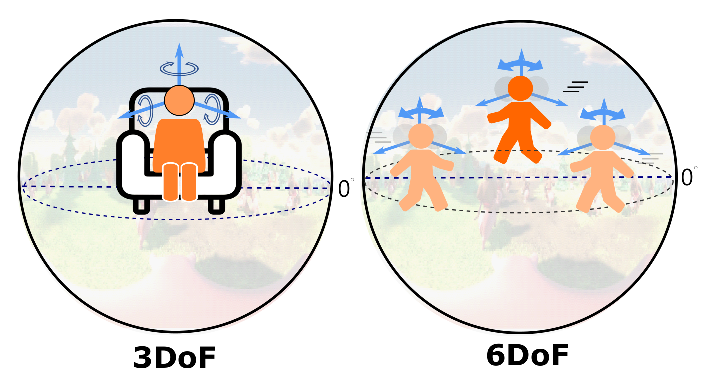
\includegraphics[width=0.46\textwidth]{figs/vr_phase}
    \caption{Difference between 3DoF and 6DoF interactions.}
    \label{fig:vr_phase}
\end{figure}

Supporting 6DoF Extended Reality (XR) using 360{\degree} videos is not an easy task, because, for every single position, a new 360{\degree} video needs to be captured.
Even if we deploy dense 360{\degree} cameras, users may still miss smooth transitions at the positions between any two adjacent cameras.
Hence, more descriptive 3D representations are required for enabling the truly immersive experience of 6DoF VR applications.
Recently, MPEG-I (Moving Picture Expert Group--Immersive Group) has been actively developing MPEG Immersive Video (MIV) standard~\cite{BDDF+21, MPEG_MIV_web} which can use for 6DoF video compression.
It uses multi-view RGB-D video as the data representation and includes the integrated pipeline for encoding, decoding, synthesizing, and rendering.
The Test Model for Immersive Video (TMIV)~\cite{tmiv_doc,tmiv_gitlab}, which is the reference software of MIV standard, has been released to show a reference implementation of MIV.

Besides, reducing bandwidth and maintaining high view quality is a bottleneck of 6DoF real-time streaming.
Because of the limitation of bandwidth, performing the best quality by adaptive quality model for 6DoF immersive video is quite a challenging work.
There are many existing rate control algorithms for video compression~\cite{PZAB16}\cite{WYTC12}\cite{HM01}.
Based on the existed rate control algorithms, it is possible to optimize those models to predict the 6DoF video performance.
Although, there are still many effects that could impact the 6DoF video quality, e.g., tile sizes~\cite{JLLR20}, camera placements, complexity of scenes~\cite{BWJ21}, number of groups, synthesizer, and a quantization parameter.
In this paper, we conduct a rate-distortion model (RD-model) to predict the performance of 6DoF immersive video in common situations as we show in Fig.~\ref{fig:RD_model_concept}.
The model will design in an empirical way and aim at some vital TMIV parameters.
The main goal of this model is to generate relevance between TMIV parameters and quality metrics, e.g., PSRN, SSIM, and VMAF.
Once the model generates, it is possible to use on estimate the 6DoF immersive video performance in different camera placements and also use it on real-time 6DoF streaming.

\begin{figure}[tbh]
    \centering
    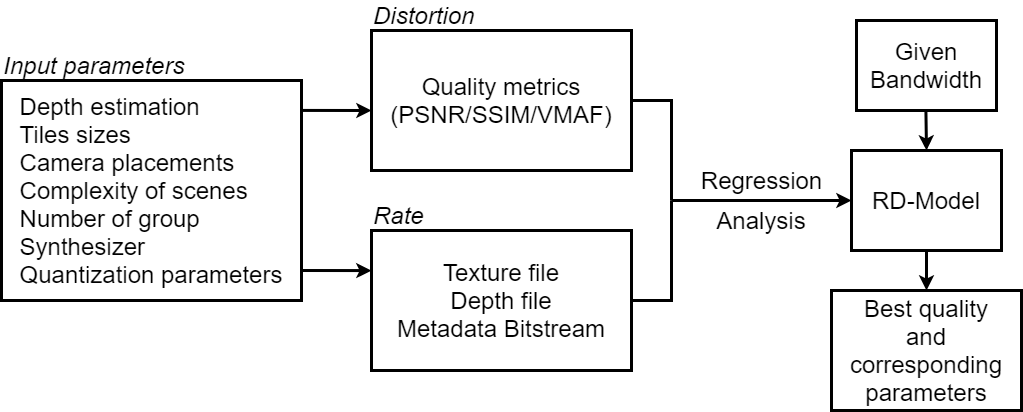
\includegraphics[width=0.46\textwidth]{figs/RD_model_concept}
    \caption{RD-model workflow}
    \label{fig:RD_model_concept}
\end{figure}

% The rest of this paper is organized as follows. We survey the related work in Sec.~\ref{sec:related}, and giving an introduction for MIV standard in Sec.~\ref{sec:TMIV}. Sec.~\ref{sec:implementation} introduce our implementation for experiments. The setup and results of our experiments are shown in Sec.~\ref{sec:experiment}. Finally, we conclude this paper and list some future work in Sec.~\ref{sec:conclusion}
